% !TeX root = ../main.tex

\chapter{系统详细设计与实现}

在前两章中完成需求分析以及系统概要设计之后,本章将详细介绍各个功能
模块重难点的设计与实现。针对每一个功能模块,首先进行功能流程描述,然后对系
统实现类进行设计并阐述,通过类图介绍系统对象之间的交互顺序,最后进行系统实现的效果图展示。

\section{数据源管理}

数据源是入湖任务的前提要求,是Iceberg入湖任务的源头,注册相应数据源,创建入湖任务时即可根据创建的数据源选择对应的源表。
从数据源分类上来看,数据湖分析系统支持关系型数据库源(mysql)以及消息队列数据源(tube、kafka、pulsar),
该模块支持数据源创建、查看、编辑、删除功能。数据源创建的相关页面如图5.1所示。

\begin{figure}[h]
  \centering
  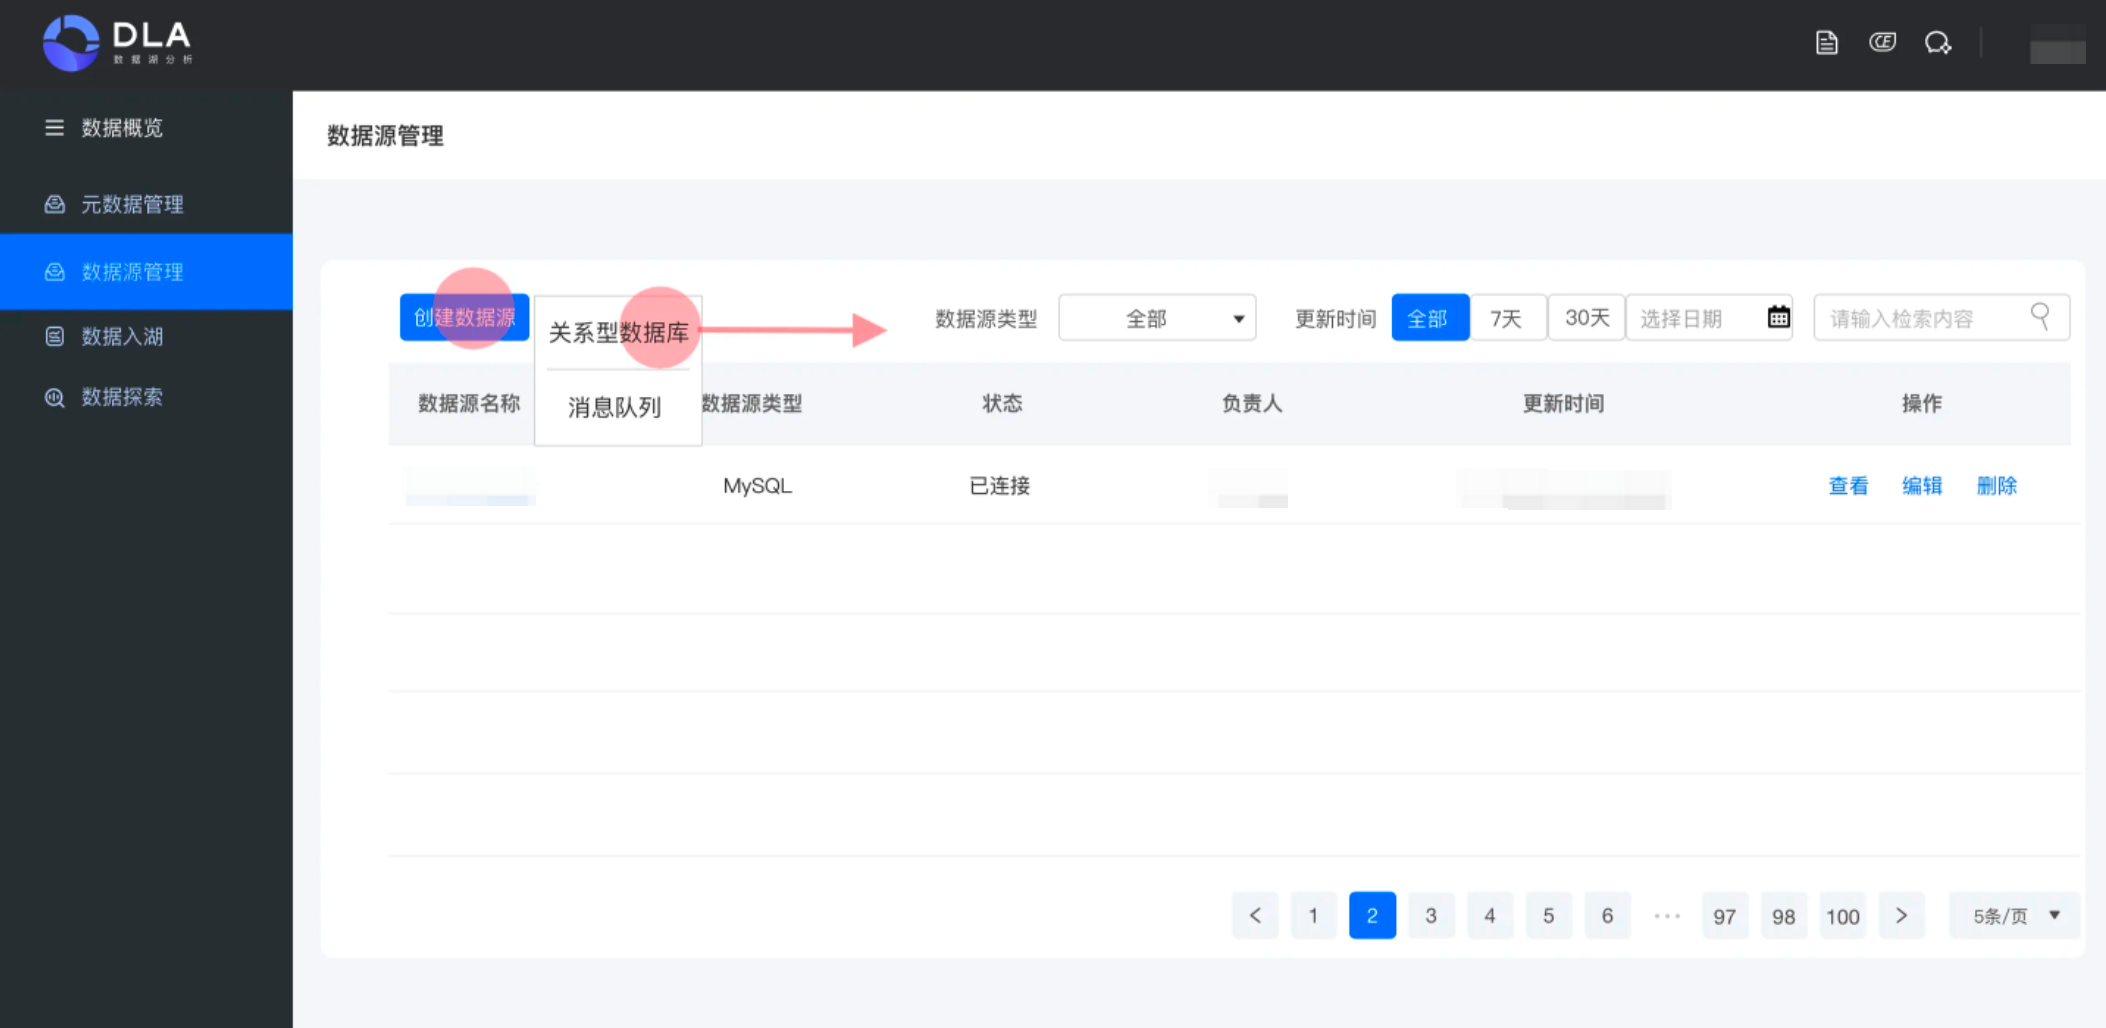
\includegraphics[width=1.0\textwidth]{创建数据源.png}
  \caption{创建数据源页面}
  \label{fig:badge}
\end{figure}

在数据源管理系统模块中,用户首先需要登录系统,通过安全中心认证服务进
行身份认证。成功登录系统之后,进行数据源信息录入,基本信息包括
数据源名称和描述,不同的数据源所需要的详细信息也不一样,以关系型数据库MySQL为例,需
要配置mysql用户名、密码、库名、服务器地址和服务器端口。完成配置信息设置之后,
会将数据源持久化保存在数据库中。流程图如图5.2所示。

\begin{figure}[h]
  \centering
  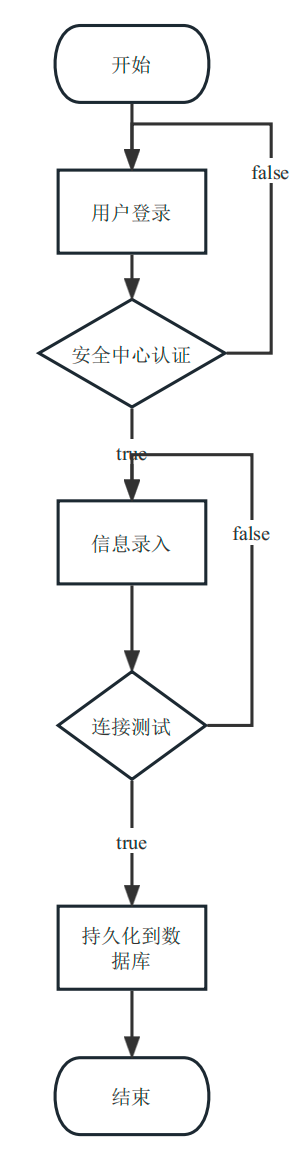
\includegraphics[width=0.3\textwidth]{创建数据源流程图.png}
  \caption{创建数据源流程图}
  \label{fig:badge}
\end{figure}

数据源管理是基于SpringBoot框架的Web应用,系统的主要类图如图5.3所示:

\begin{figure}[h]
  \centering
  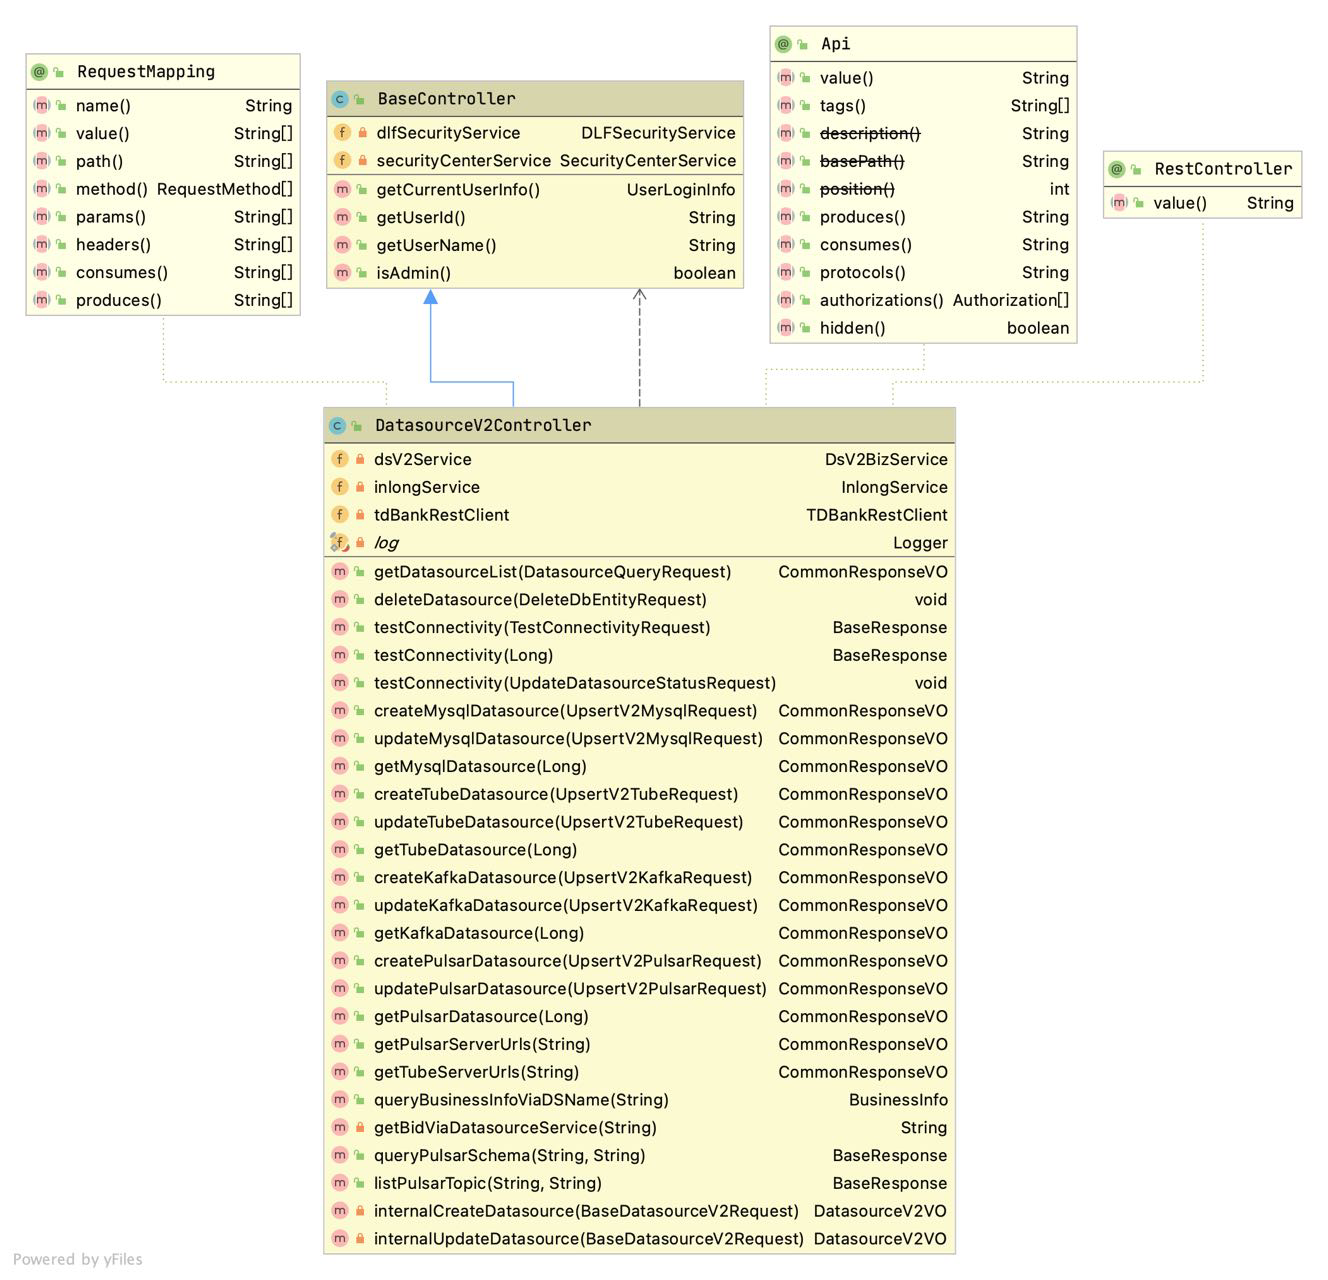
\includegraphics[width=1.0\textwidth]{数据源类图.png}
  \caption{数据源管理类图}
  \label{fig:badge}
\end{figure}

DatasourceV2Controller是数据源管理模块的核心类,是用户访问数据源管理的入口,
主要负责接受各种数据源的创建、查看、更新、删除以及连接测试的请求,对应的逻辑处理是在
成员变量DsV2BizService中实现的。

\section{元数据管理}

元数据是描述其他数据的数据,它提供有关信息资源的结构数据。它用于识别、
评价和追踪资源,实现简单高效地管理大量网络化数据,并有效地发现、查找、组织和管理信息资源。

这里的元数据是描述Iceberg表的,Iceberg表即目标表,
是入湖任务的前提要求,可以创建新表或关联已有的表。元数据管理模块主要管理Iceberg元数据,
包括数据优化、表的创建、编辑和查看四个主要功能。其中数据优化功能将单独介绍。表的创建可在数据湖分析
系统上创建新的Iceberg表,也可以关联在其他平台上已创建的Iceberg表。表的编辑支持对已创建的表进行
修改和编辑,包括增加和删除字段操作。元数据管理的相关页面如图5.4所示。

\begin{figure}[h]
  \centering
  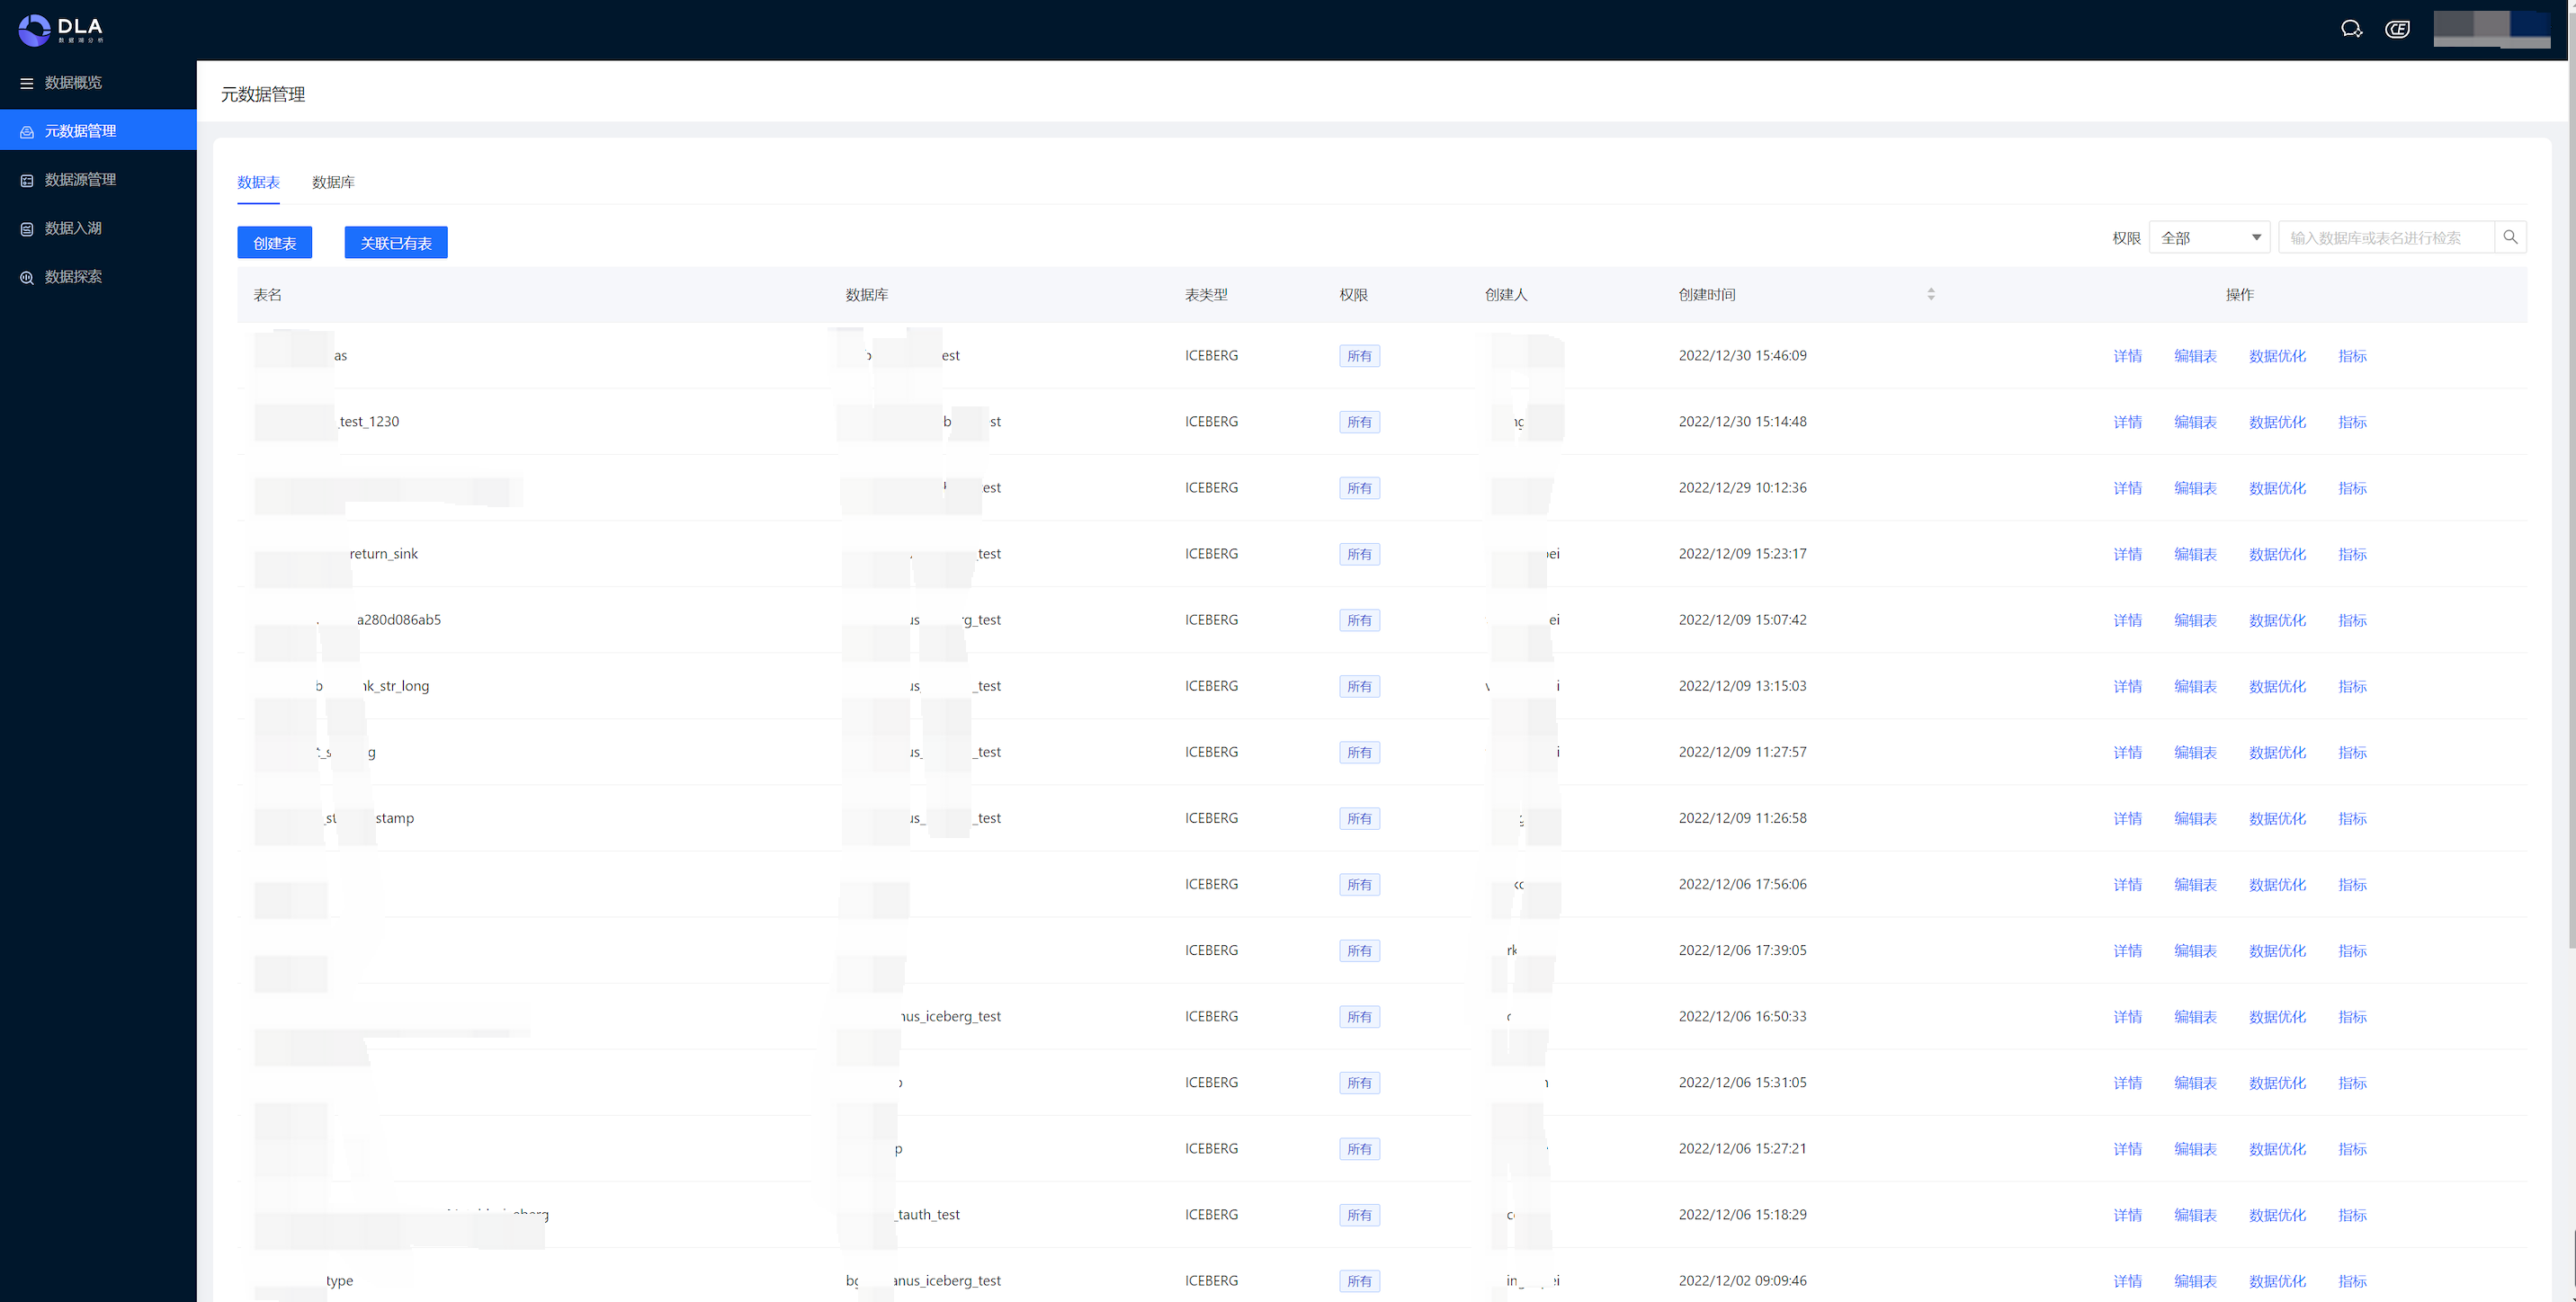
\includegraphics[width=1.0\textwidth]{元数据管理.png}
  \caption{元数据管理页面}
  \label{fig:badge}
\end{figure}

在元数据管理系统模块中,用户在对元数据进行操作前,都必须通过安全中心认证服务,
因为Iceberg元数据是存储在hive metastore中的,而对hive metastore中的元数据修改在企业内
是比较敏感的,所以必须添加身份认证以及权限认证来确保安全问题。
以Iceberg表的创建和修改来说,表的创建需要和hive metastore、mysql进行交互,一个createTable的request建立后,首先会判断
metastore中是否已存在表,若不存在,则会判断MySQL中是否存在对应的DB和table,这里MySQL中的DB和
table实质上是一个映射,是用来方便在数据湖分析系统中展示表元数据的,若MySQL中不存在,则创建对应的DB和table,
接着会在hive metastore中创建实际的Iceberg表元数据,表的修改如果涉及到字段的增加及删除操作,则会更新hive metastore中对应的表元数据。
这其中涉及到的对hive metastore进行操作前都会进行安全中心的身份认证和权限认证。流程图如图5.5所示。

\begin{figure}[h]
  \centering
  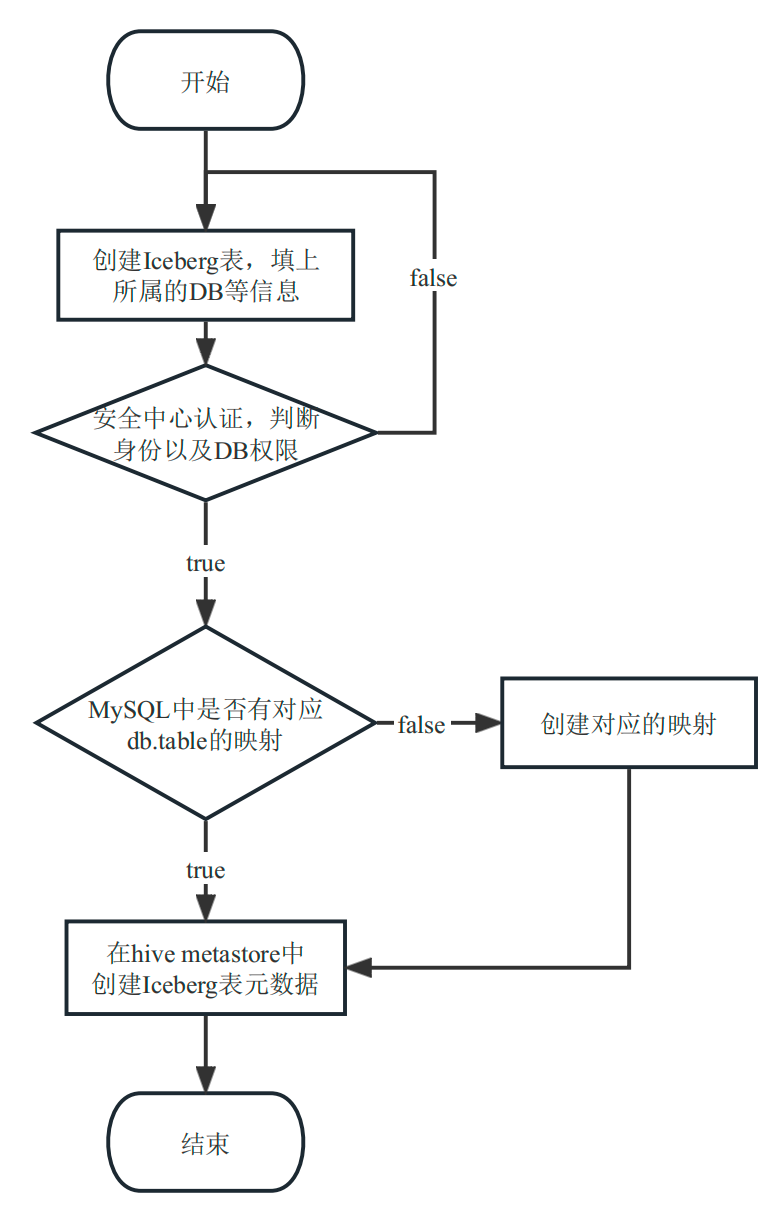
\includegraphics[width=0.5\textwidth]{表元数据创建流程图.png}
  \caption{Iceberg表元数据创建流程图}
  \label{fig:badge}
\end{figure}

元数据管理系统中主要类图如图5.6所示:

\begin{figure}[h]
  \centering
  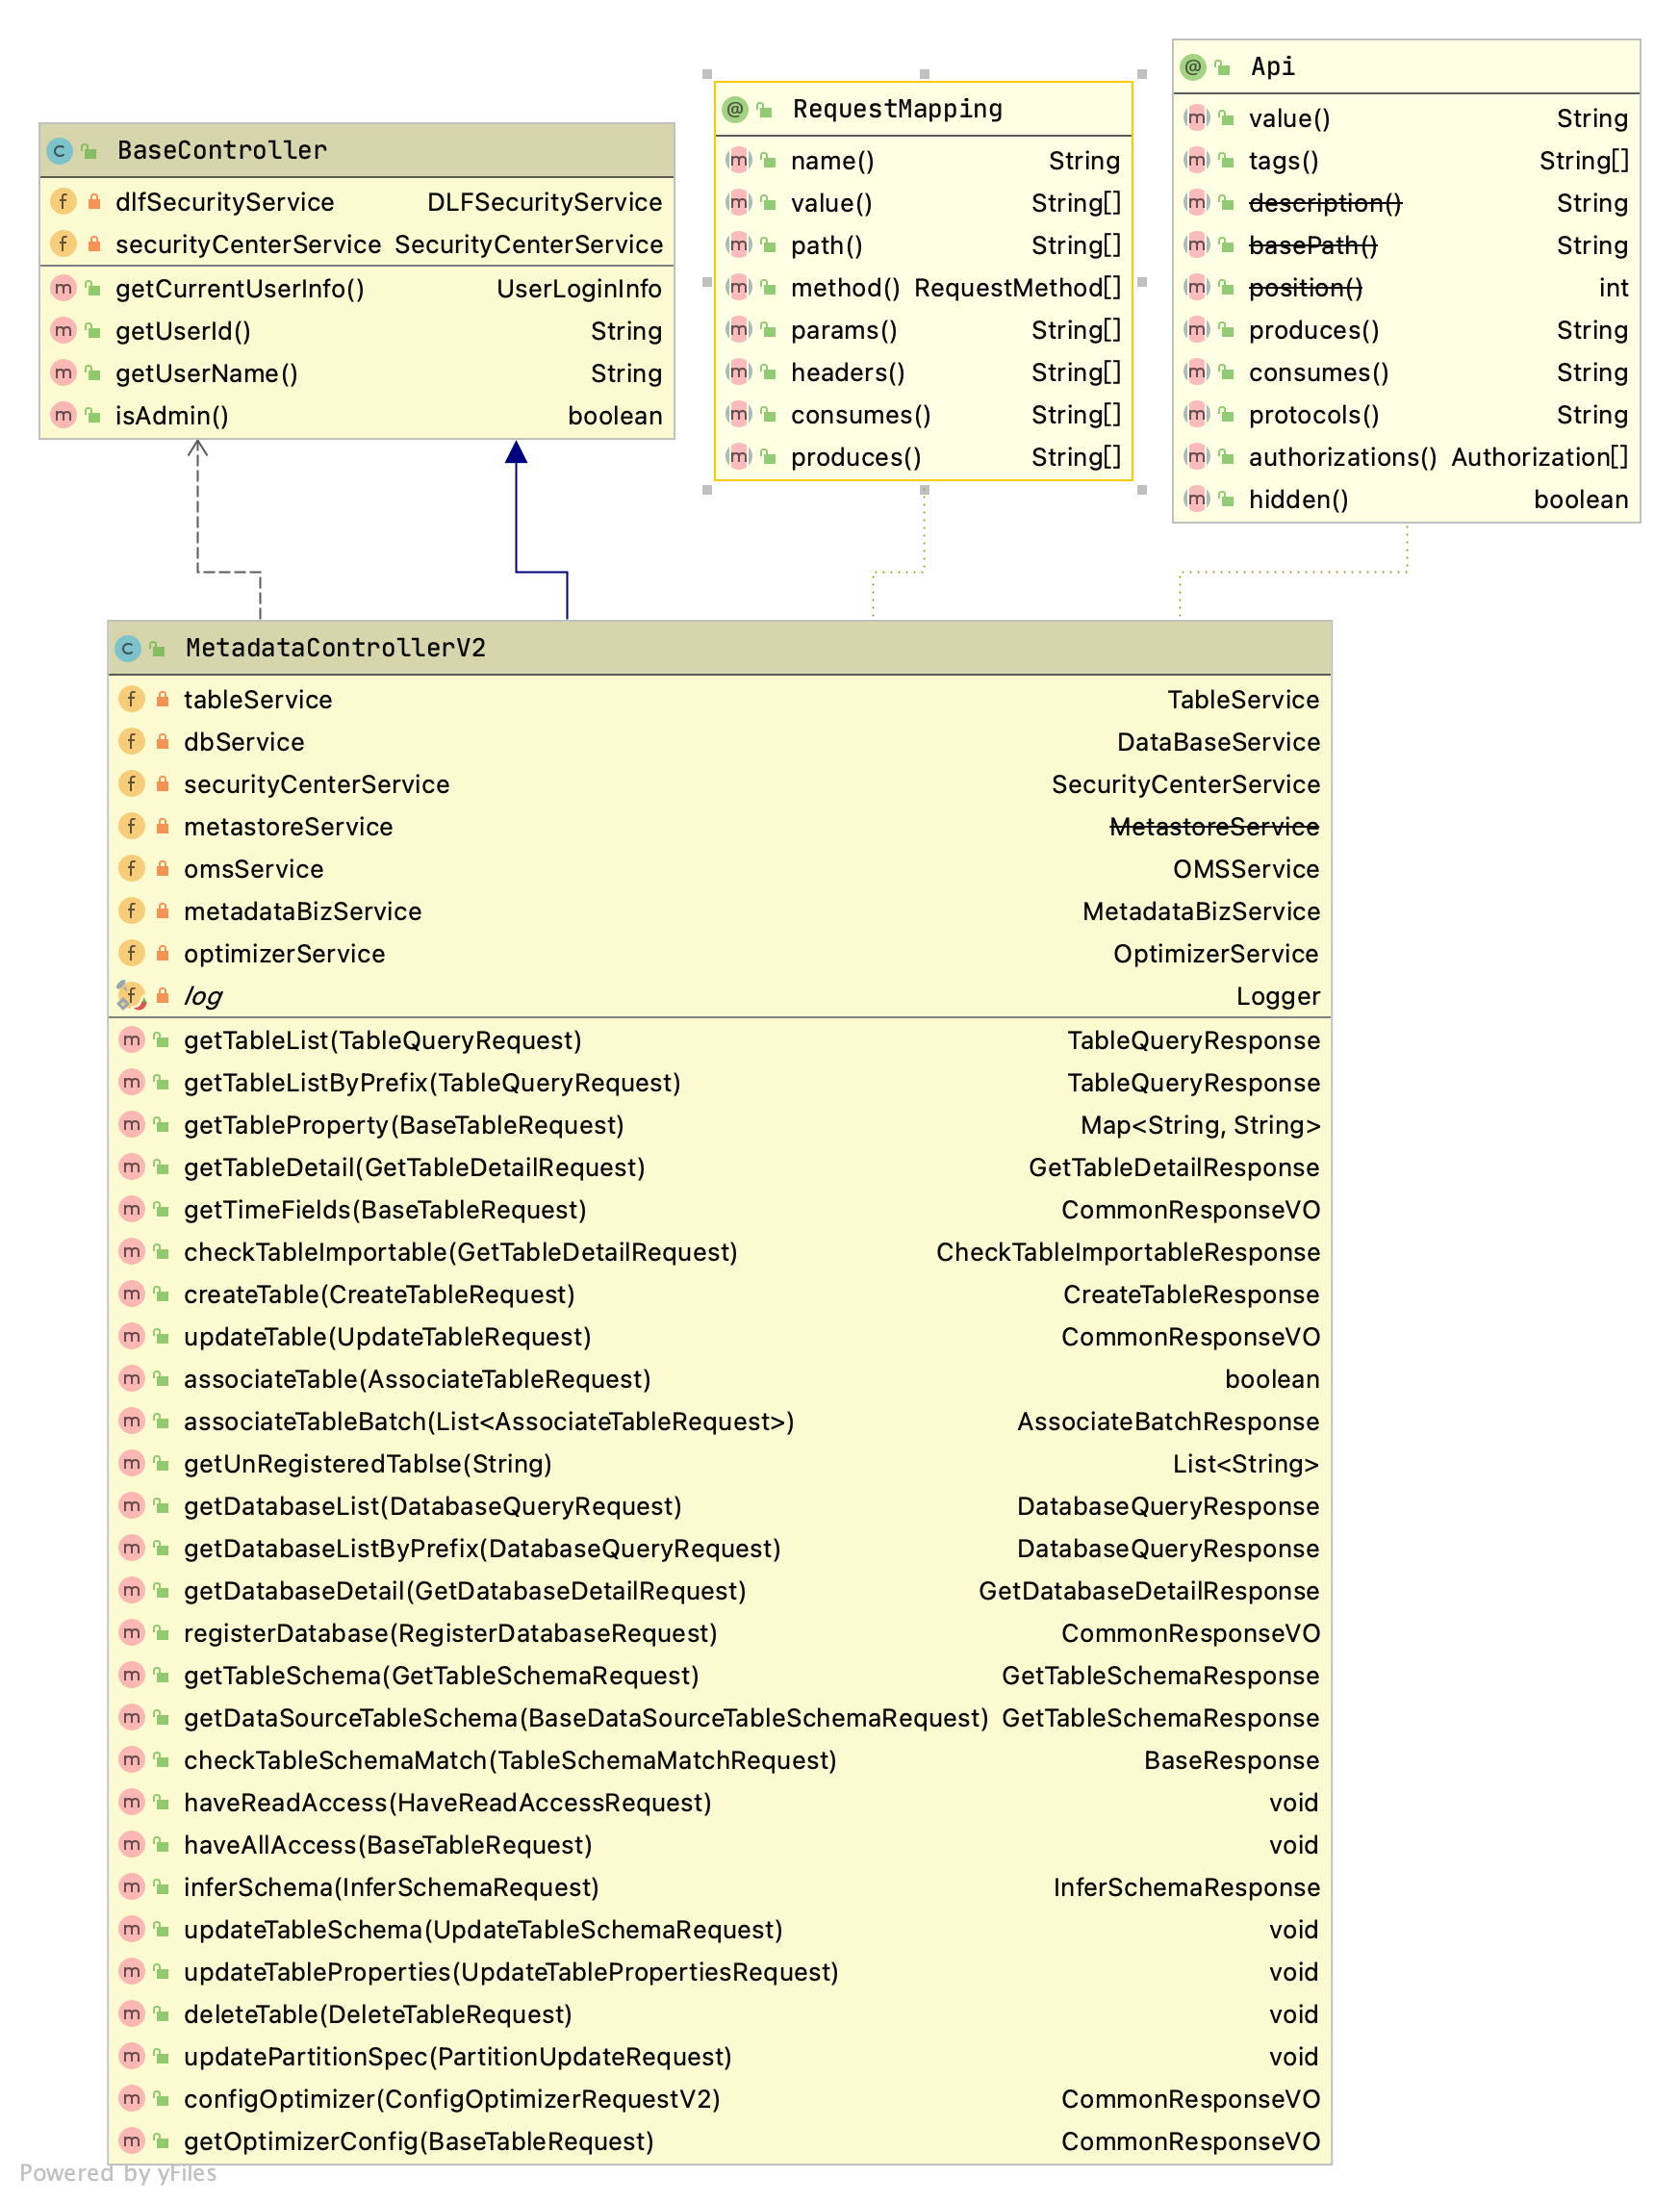
\includegraphics[width=1.0\textwidth]{MetadataControllerV2.png}
  \caption{元数据管理类图}
  \label{fig:badge}
\end{figure}

MetadataControllerV2是元数据管理的核心类,是用户访问元数据管理的入口,
主要负责Iceberg表的创建、修改、查看、数据优化等功能。在核心类的成员变量中,
TableService负责Iceberg表的创建、修改、查看的逻辑处理;DataBaseService
负责数据库相关操作的逻辑处理;SecurityCenterService负责安全中心认证的逻辑处理,
安全中心认证是所有操作元数据的前提,必须通过认证后,才能对表的结构以及数据进行查看或者修改;
OMSService是元数据服务,是基于hive metastore实现的;
OptimizerService是表的自动优化的逻辑处理,会在后面进行详细介绍。


\section{数据入湖}

数据入湖功能模块是DLA系统核心流程功能,目的是用户通过该功能将源数据表流程化入湖
以及查看已申请入湖任务执行情况。其中入湖任务列表中具有操作任务的功能,
并且根据数据入湖方式具有不同状态展示,以供用户查看和处理。入湖任务列表如图5.7所示。

\begin{figure}[h]
  \centering
  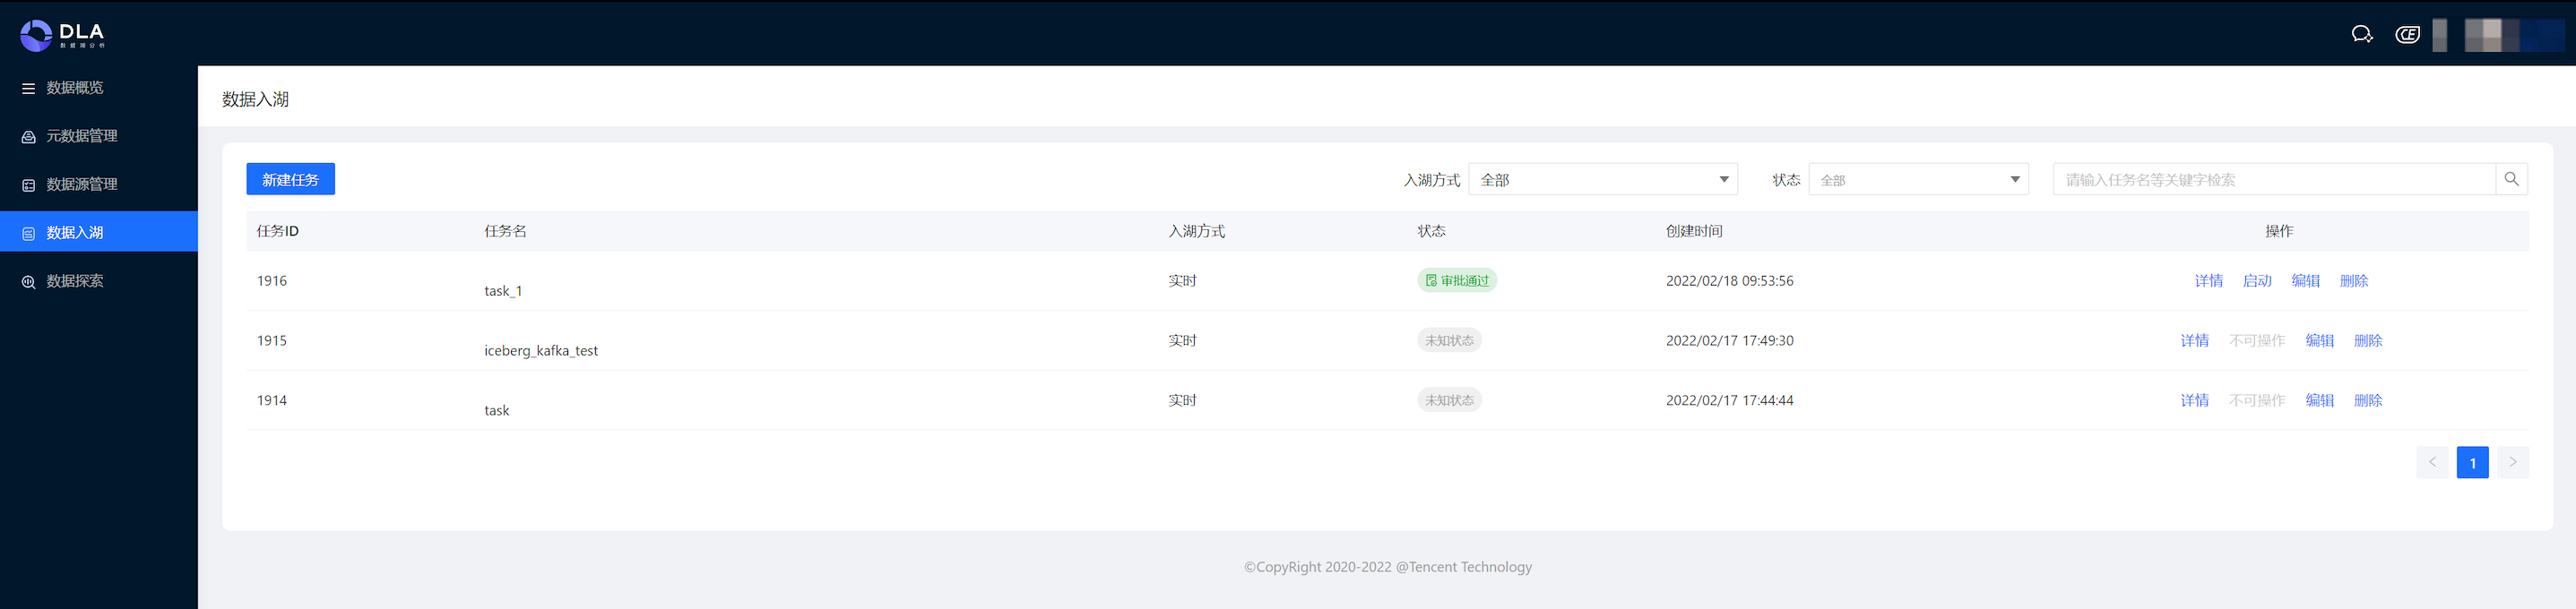
\includegraphics[width=1.0\textwidth]{数据入湖.png}
  \caption{数据入湖列表}
  \label{fig:badge}
\end{figure}

对于每一个入湖任务,都需要进行五步。
第一步是进行基础信息的填写,根据入湖需要选择对应的任务类型,填写必要的任务名;
第二步是填写源表的信息,其中实时入湖与关系型数据库入湖需要提前注册数据源,选择对应数据源表;
第三步是填写目标表的信息,若目标表已经创建,则会自动填充信息,若不存在,则会自动创建Iceberg表,无需提前新建表,这大大优化了入湖任务的流程;
第四步是进行映射预览,会对源表及目标表的schema进行比对,若schema不一致将无法进行下一步;
第五步是配置参数及资源。相关的流程图如图5.8所示。

\begin{figure}[h]
  \centering
  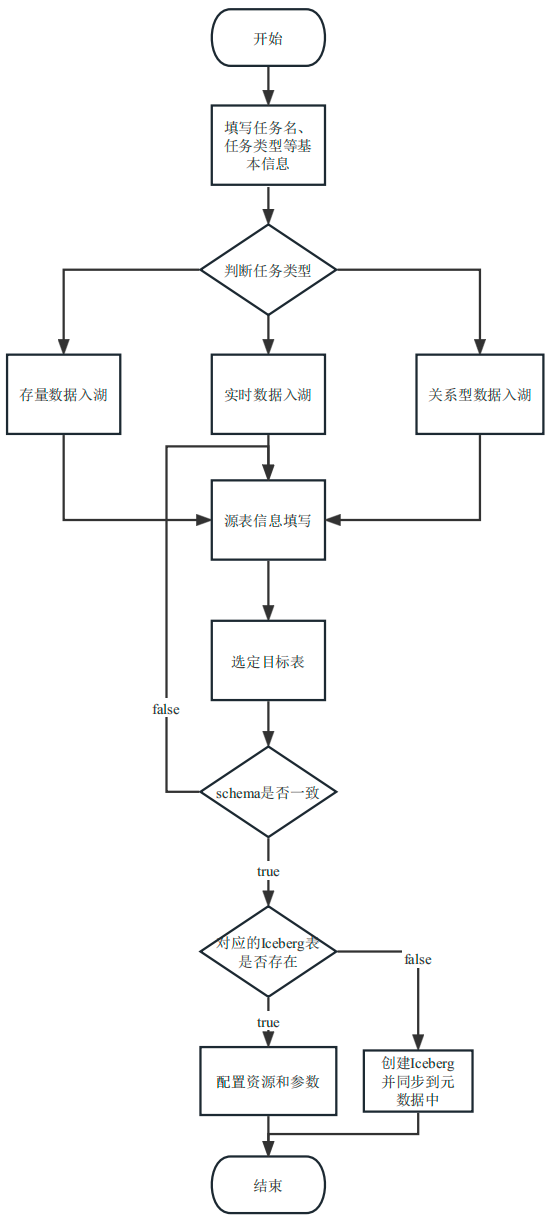
\includegraphics[width=0.5\textwidth]{任务创建流程图.png}
  \caption{入湖任务创建流程图}
  \label{fig:badge}
\end{figure}

针对不同的任务类型,我们分别对接了内部的不同任务平台,通过各个平台的REST API的方式实现不同任务的创建。
若为实时数据入湖任务,则会在实时流计算平台Oceanus上创建对应的实时任务来进行Iceberg表的写入,
Oceanus底层使用的引擎是flink;若为存量数据入湖或者关系
型数据入湖,则会在统一调度平台US上创建定时任务来进行Iceberg表的写入,底层使用的引擎是spark,
并且可在系统上设置时间间隔和起始时间。相关的核心类图如图5.9所示。

\begin{figure}[h]
  \centering
  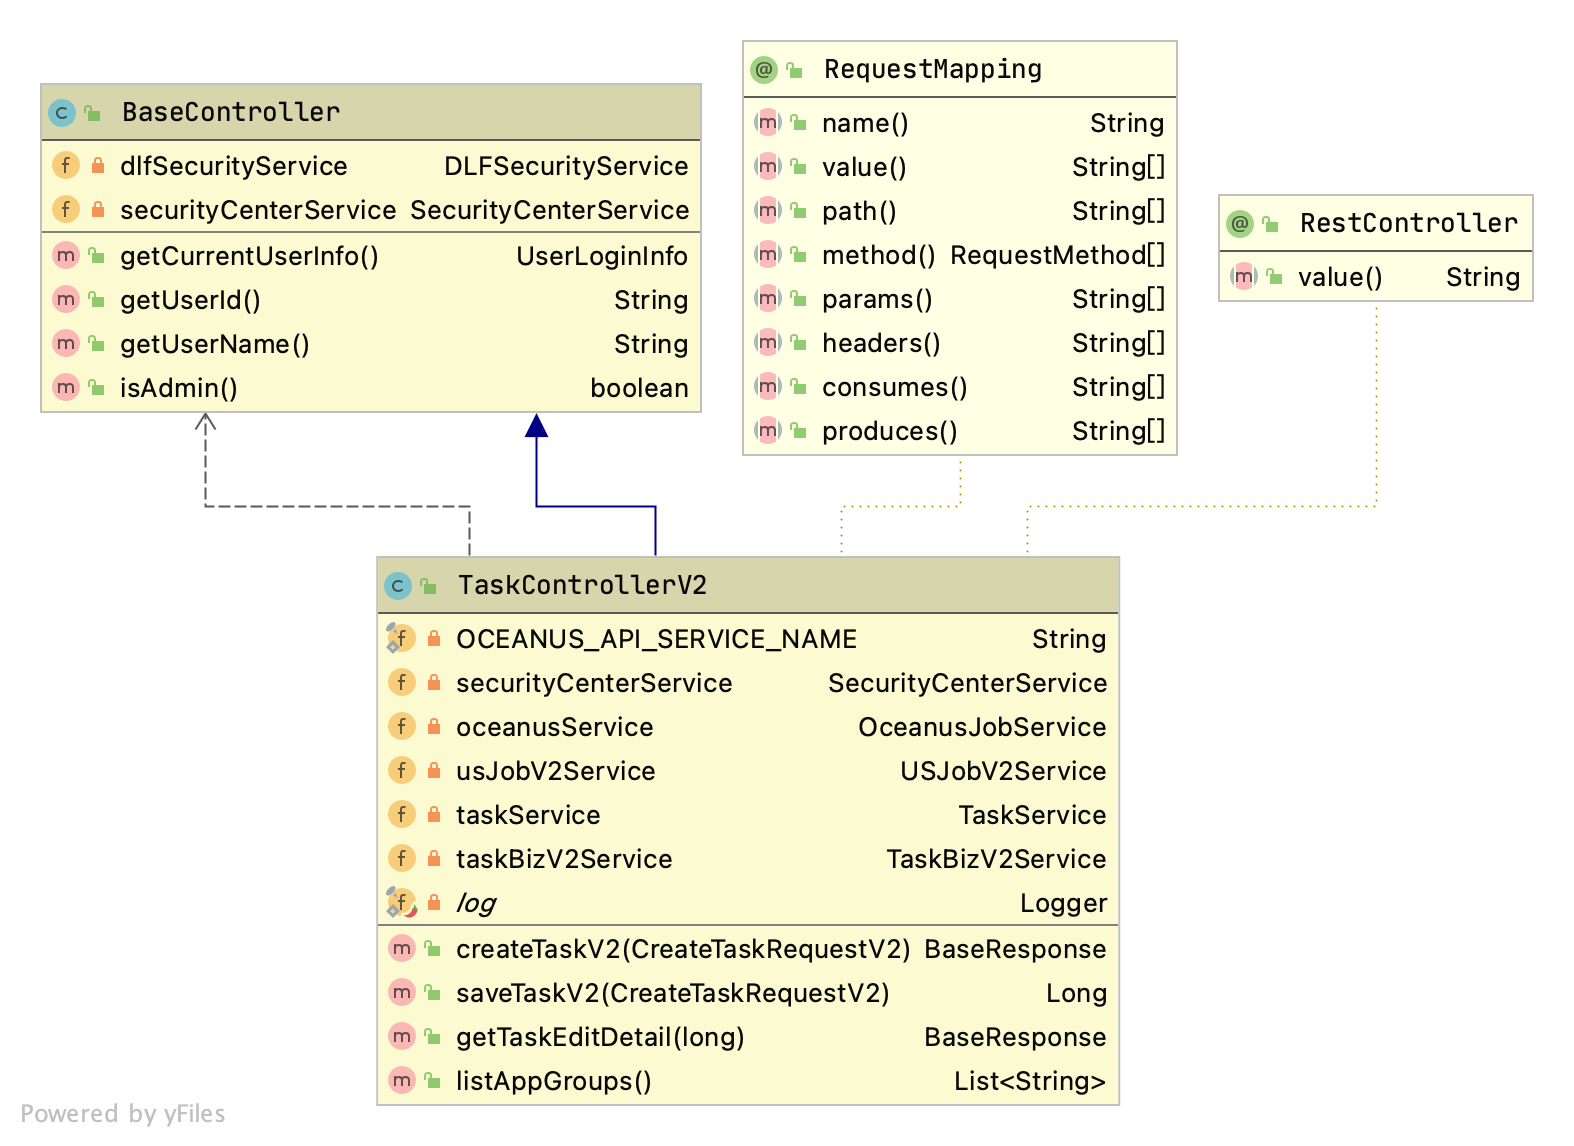
\includegraphics[width=1.0\textwidth]{TaskControllerV2.png}
  \caption{数据入湖类图}
  \label{fig:badge}
\end{figure}

可以看到,TaskControllerV2是数据入湖管理的核心类,是用户进行任务创建的入口,负责入湖任务的
创建、查看修改等功能,对应的逻辑处理是在TaskBizV2Service中实现的。在成员变量中,SecurityCenterService
是负责安全中心认证的;OceanusJobService是负责管理实时任务的,对接的是实时任务平台的api;
USJobV2Service是负责管理存量数据入湖任务的,对接的是统一调度平台US的api。

\section{数据探索}

数据探索是数据入湖后,用户需要进行数据查看或者数据分析时使用的工具,目前主要依赖内部的统一查询平台实现数据探索功能,
通过查询平台的SuperSQL,用户只需简单的配置参数(set supersql.execution.engine = presto / spark),
就可以轻松通过Presto或者Spark查询分析数据。SuperSQL做到计算对用户透明,
避免用户在不同系统中的切换成本和高昂的学习成本。SQL语法采用标准的SQL语法。例如图5.10。
除了可以使用标准的sql进行数据探索外,统一查询平台还提供了Jupyter Notebook的方式,可以在Jupyter中使用Pyspark进行
数据的探索,该种方式与用户的交互性比较好,可以使用各种图表使数据可视化。

\begin{figure}[h]
  \centering
  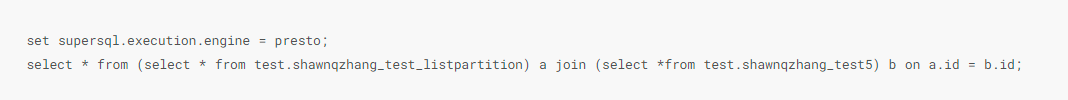
\includegraphics[width=1.0\textwidth]{presto标准sql.png}
  \caption{Presto查询sql}
  \label{fig:badge}
\end{figure}

除了内部的统一查询平台可以进行数据探索外,我们还在数据湖分析平台中内嵌了Zeppelin来提供数据探索。
Zeppelin是一个基于Web的notebook,提供交互数据分析和可视化。后台支持接
入多种数据处理引擎,如spark,hive等。支持多种语言: Scala(Apache Spark)、
Python(Apache Spark)、SparkSQL、 Hive、 Markdown、Shell等。
开发者可以通过实现更多的解释器来为Zeppelin添加数据引擎。Zeppelin的使用页面如图5.11所示。

\begin{figure}[h]
  \centering
  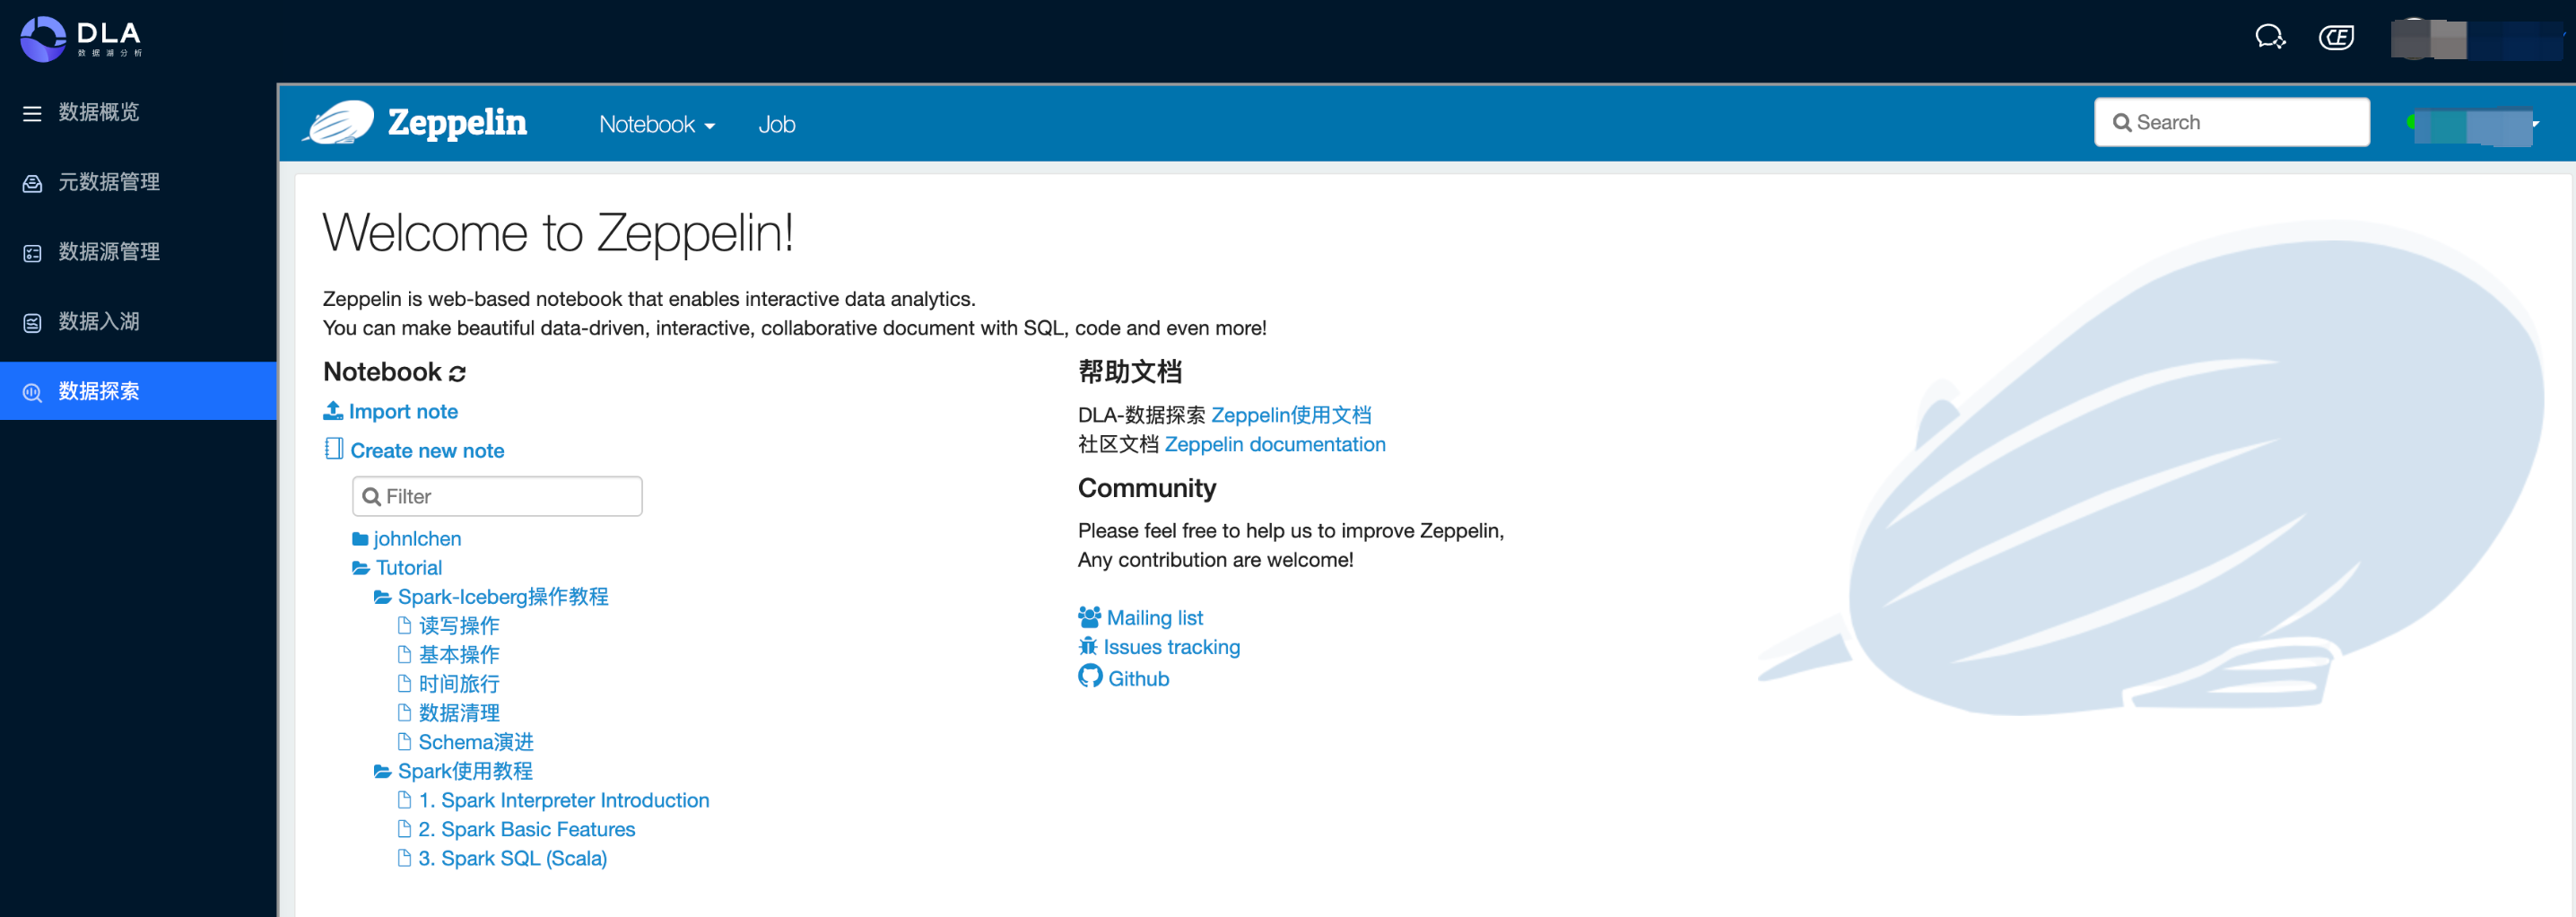
\includegraphics[width=1.0\textwidth]{Zeppelin使用.png}
  \caption{Zeppelin使用页面}
  \label{fig:badge}
\end{figure}

\section{自动优化服务}



\subsection{合并小文件}



\subsection{清理过期快照数据}



\subsection{删除孤儿文件}



\subsection{生命周期管理}



\section{本章小结}


